%% memorygraphs.tex
%% Copyright 2018-2019 C. Staps
%
% This work may be distributed and/or modified under the
% conditions of the LaTeX Project Public License, either version 1.3
% of this license or (at your option) any later version.
% The latest version of this license is in
%   http://www.latex-project.org/lppl.txt
% and version 1.3 or later is part of all distributions of LaTeX
% version 2005/12/01 or later.
%
% This work has the LPPL maintenance status “maintained”.
%
% The Current Maintainer of this work is C. Staps.
%
% This work consists of the files memorygraphs.sty and the documentation in
% memorygraphs.tex and example-fibonacci.tex.
\documentclass[a4paper]{article}

\usepackage{geometry}
\usepackage[hidelinks]{hyperref}
\usepackage{csquotes}
\usepackage{cleveref}

\usepackage[nonewpage]{imakeidx}
\makeindex[intoc]

\usepackage{latexgit}
\usepackage{fancyvrb}
\usepackage{listings}
\usepackage{color}
\definecolor{codebg}{rgb}{0.8,0.8,1}
\lstset{backgroundcolor=\color{codebg},
	frame=single,
	framerule=0pt,
	basicstyle=\ttfamily\footnotesize,
	columns=fullflexible}

\usepackage{memorygraphs}

\newcommand{\memorygraphs}{\textsf{memorygraphs}}
\newcommand{\TikZ}{Ti\textit{k}Z}

\title{The \memorygraphs{} package}
\author{Camil Staps\thanks{info@camilstaps.nl}}
\date{\gitcommitdate[formatDate]}

\newif\ifexamplehorizontal
\newenvironment{example}{%
		\medskip%
		\VerbatimOut{\jobname.tmp}}
	{\endVerbatimOut%
		\ifexamplehorizontal%
			\noindent\begin{minipage}{\linewidth}
				\centering
				\input{\jobname.tmp}
			\end{minipage}
			\par\bigskip
			\noindent\begin{minipage}{\linewidth}
				\lstinputlisting{\jobname.tmp}
			\end{minipage}
		\else%
			\hfill%
			\noindent\begin{minipage}{.4\linewidth}
				\centering
				\input{\jobname.tmp}
			\end{minipage}%
			\noindent\begin{minipage}{.6\linewidth}
				\lstinputlisting{\jobname.tmp}
			\end{minipage}
		\fi%
	}

\makeatletter
\definecolor{keyheading}{rgb}{0.75,0,0}
\newcommand{\keyheading}[2][\pgfutil@empty]{%
	\index{#2@\texttt{#2} key}%
	\edef\pgf@test{#1}%
	\item\texttt{{\color{keyheading}{/tikz/#2}}\ifx\pgf@test\pgfutil@empty\else\,=\,#1\fi}\par}
\newenvironment{keydescription}[2][\pgfutil@empty]{%
		\list{}{\leftmargin=2em\itemindent-\leftmargin}
		\itemsep=0pt
		\parskip=0pt
		\topsep=0pt
		\keyheading[#1]{#2}
	}{\endlist}
\newenvironment{macrodescription}[2][\pgfutil@empty]{%
		\index{#2@\texttt{\textbackslash{}#2}}%
		\list{}{\leftmargin=2em\itemindent-\leftmargin}
		\itemsep=0pt
		\parskip=0pt
		\topsep=0pt
		\item\texttt{{\color{keyheading}{\textbackslash#2}}\,#1}
		\par\parskip3pt
	}{\endlist}
\newcommand{\marg}[1]{\texttt{\textbraceleft}$#1$\texttt{\textbraceright}}
\makeatother

\newcommand{\opt}[1]{$\langle#1\rangle$}

\begin{document}

\maketitle

\begin{center}
\input{example-fibonacci}
\end{center}

\tableofcontents

\section{Introduction}
This is the documentation of the \LaTeX{} package \memorygraphs{}.
It defines some \TikZ{} styles and adds anchors to existing styles that ease the declaration of \enquote{memory graphs}.
It is intended for graphs that represent the memory of a computer program during its execution.

\section{Functionality}

\begin{keydescription}{memory graph}
The \verb$memory graph$ style is to be used on \verb$tikzpicture$.
It sets a different node distance that the author finds suitable for this kind of graphs.

\begin{example}
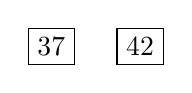
\begin{tikzpicture}[memory graph]
  \node[draw] (x) {37};
  \node[draw,right=of x] {42};
\end{tikzpicture}
\end{example}
\end{keydescription}

\subsection{Nodes}
The following styles can be used to typeset memory blocks:

\begin{keydescription}{block}
This is the most basic style to define a memory block.
By default, this shape is a rectangle with borders:

\begin{example}
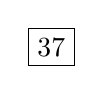
\begin{tikzpicture}[memory graph]
  \node[block] {37};
\end{tikzpicture}
\end{example}
\end{keydescription}

\begin{keydescription}[\opt{n}]{arity}
The \verb$arity$ style can be used to create a node with arguments.
This implies \verb$block$:

\begin{example}
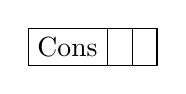
\begin{tikzpicture}[memory graph]
  \node[arity=2] {Cons};
\end{tikzpicture}
\end{example}
\end{keydescription}

\begin{macrodescription}[\marg{i}]{arg}
Because blocks with \verb$arity$ are multipart rectangles,
	one can use \TikZ{}'s \verb$\nodepart$ to put contents in the arguments.
However, it can be confusing that \verb$\nodepart{two}$ refers to the \emph{first} argument,
	so we redefine \verb$\arg$ in \verb$block$s to identify arguments of the memory block:

\begin{example}
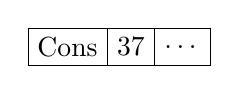
\begin{tikzpicture}[memory graph]
	\node[arity=2] {Cons \arg{1} 37 \arg{2} \dots};
\end{tikzpicture}
\end{example}

Should one want to use math mode's \verb$\arg$ in a memory block, they can first rename it:

\begin{example}
\let\matharg\arg
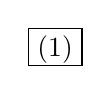
\begin{tikzpicture}[memory graph]
  \node[block] {$\matharg(1)$};
\end{tikzpicture}
\end{example}
\end{macrodescription}

\subsection{Markings}
It is possible to mark the head of memory blocks using triangles in the north east and south east corners.

\begin{keydescription}[\opt{style}]{block mark north east}
\keyheading[\opt{style}]{block mark north west}
\keyheading[\opt{style}]{block mark south east}
\keyheading[\opt{style}]{block mark south west}
With this key, triangular marks can be added to the corners of the head of a node:

\begin{example}
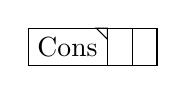
\begin{tikzpicture}[memory graph]
  \node[arity=2,block mark north east] {Cons};
\end{tikzpicture}
\end{example}

It is optional to add a style:

\begin{example}
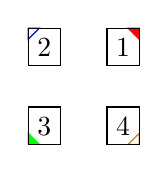
\begin{tikzpicture}
    [memory graph,every node/.style={block}]
  \node[block mark north east={fill,red}] at (1,1) {1};
  \node[block mark north west={blue}] at (0,1) {2};
  \node[block mark south west={fill,green}] at (0,0) {3};
  \node[block mark south east={brown}] at (1,0) {4};
\end{tikzpicture}
\end{example}

The key is long to avoid clashes with other packages,
	and because it depends on the context what nodes should be marked for.
It is of course possible to define a shorthand in your own document.
One application is to mark nodes that are in head normal form (HNF),
	for which one may define the key \verb$hnf$:

\begin{example}
\tikzset{every block/.style={block mark south east}}
\tikzset{hnf/.style={block mark south east=fill}}
\begin{tikzpicture}[memory graph]
  \node[arity=2,hnf]
    {Cons \arg{1}$\dots$ \arg{2}$\dots$};
  \node[arity=2] at (0,-1)
    {map \arg{1}$\dots$ \arg{2}$\dots$};
\end{tikzpicture}
\end{example}

The size of the rectangles is defined by \verb$\memorygraphs@marklength$,
	which can of course be changed.
The default is \makeatletter\the\memorygraphs@marklength\makeatother.

\begin{example}
\makeatletter
\memorygraphs@marklength=7pt
\makeatother
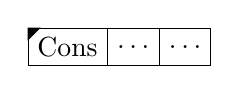
\begin{tikzpicture}[memory graph]
  \node[arity=2,block mark north west=fill]
    {Cons \arg{1}$\dots$ \arg{2}$\dots$};
\end{tikzpicture}
\end{example}
\end{keydescription}

\subsection{Anchors}
\index{anchors}
Because blocks with \verb$arity$ are multipart rectangles,
	one can use anchors like \verb$two south$ to refer to the south of the second part of a node.
These are aliased as \texttt{arg $i$ south} (and similar for other anchors on multipart nodes),
	where \verb$arg 1$ stands for \verb$two$.
The first block of a node is aliased as \verb$head$ instead of \verb$arg 0$,
	so one can use \verb$head south$.
For \verb$head$, anchors for the corners (\verb$head north east$, etc.) are defined as well.

The parts of multipart rectangles do not normally have a \verb$center$ anchor, but \memorygraphs{} defines these.
One can use both \verb$two center$ and \verb$arg 1 center$ to refer to the center of the first argument of a node.

The additional anchors are shown below.
See the \TikZ{} manual for the predefined anchors.

{\examplehorizontaltrue
\begin{example}
\Large
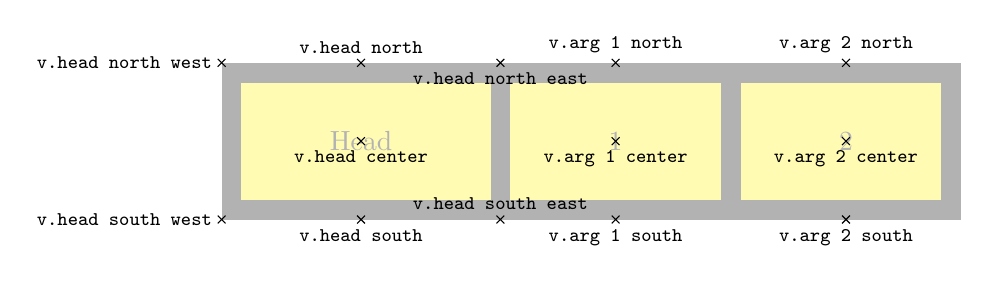
\begin{tikzpicture}
  \node
    [arity=2,
     line width=.25cm,inner xsep=1.25cm,inner ysep=.75cm,
     color=black!30,fill=yellow!30]
    (v) {Head \arg{1} 1 \arg{2} 2};
  \foreach \anchor/\placement in
    {head north/above,head south/below,head center/below,
     head north east/below,head south east/above,head north west/left,head south west/left,
     arg 1 north/above,arg 1 south/below,arg 1 center/below,
     arg 2 north/above,arg 2 south/below,arg 2 center/below}
    \draw[shift=(v.\anchor)] plot[mark=x] coordinates{(0,0)}
       node[\placement] {\scriptsize\texttt{v.\anchor}};
\end{tikzpicture}
\end{example}
}

\subsection{References}

\begin{keydescription}{ref}
This is a simple style for arrows with a circle at the start and slightly rounded corners:

\begin{example}
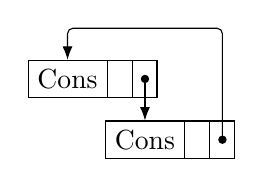
\begin{tikzpicture}[memory graph]
  \node[arity=2] (hd) {Cons};
  \node
    [arity=2,below=of hd.arg 2 center,anchor=head north]
    (tl) {Cons};
  \draw[ref] (hd.arg 2 center)
    -- (tl.head north);
  \draw[ref] (tl.arg 2 center)
    |- ($(hd.head north)+(0,.4)$)
    -- (hd.head north);
\end{tikzpicture}
\end{example}
\end{keydescription}

\section{Examples}
\examplehorizontaltrue

\begin{itemize}
\item
The linked list of Fibonacci numbers on the title page was generated with:

\noindent\begin{minipage}{\linewidth}
	\centering
	\input{example-fibonacci.tex}
\end{minipage}
\par\bigskip
\noindent\begin{minipage}{\linewidth}
	\lstinputlisting{example-fibonacci.tex}
\end{minipage}

\item
A cyclical linked list, with unboxed integers:

\begin{example}
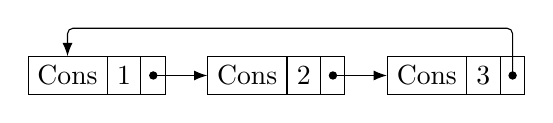
\begin{tikzpicture}[memory graph]
  \node[block,arity=2] (xs) {Cons \arg{1} 1};

  \node[block,arity=2,right=of xs.arg 2 east] (xsb) {Cons \arg{1} 2};
  \draw[ref] (xs.arg 2 center) -- (xsb);

  \node[block,arity=2,right=of xsb.arg 2 east] (xsc) {Cons \arg{1} 3};
  \draw[ref] (xsb.arg 2 center) -- (xsc);

  \draw[ref] (xsc.arg 2 center) -- +(0,.6) -| (xs.head north);
\end{tikzpicture}
\end{example}
\end{itemize}

\printindex

\end{document}
